% Completa los datos convenientemente en las zonas marcadas con TODO

\documentclass{beamer}
%PARA VISUALIZAR PRESENTACIONN CON NOTAS USAR VISUALIZADOR "pdfpc":
%Para ver las notas, el cronometro y siguente diapo:
% pdfpc --notes=right slides.pdf
% "tecla p": para pausar el cronometro
\mode<presentation> {
  \usetheme{CambridgeUS}
  \usecolortheme{crane} % color naranja
}
\setbeamercolor{titlelike}{parent=structure,bg=yellow!85!orange} % Cambia el color de la caja del título de la página inicial

\setbeamertemplate{navigation symbols}{} % ocultar iconos de navegación
\setbeamerfont{subsection in toc}{size=\small} % reducir tamaño en TOC
\setbeamerfont{date}{size=\tiny}



\usepackage[spanish]{babel}
\usepackage[utf8]{inputenc}
\usepackage{graphicx}
\usepackage{booktabs}
\usepackage{hyperref}
\usepackage{multicol}
\usepackage{pgfpages}
\usepackage{listings}
\usepackage{multimedia}
\usepackage[export]{adjustbox}
\usepackage{outlines} % Para poner bullets tabulados (\1 \2 \3 ...) y no items

\usepackage{array,tabularx} % para tabular leyenda de ecuaciones
\newenvironment{conditions*} % entorno de "leyenda de ecuación"
  {\par\vspace{\abovedisplayskip}\noindent
   \tabularx{\columnwidth}{>{$}l<{$} @{\ : } >{\raggedright\arraybackslash}X}}
  {\endtabularx\par\vspace{\belowdisplayskip}}
  
% USO DE NOTAS
\setbeameroption{hide notes} % Para mostrar u ocultar (hide/show) DESACTIVAR PARA VER NOTAS
%\setbeameroption{show only notes} % Mostrar solo las notas ACTIVAR PARA VER NOTAS
%\setbeameroption{show notes on second screen=right} % Mostrar notas en otra pantalla
%\setbeamertemplate{note page}{ % asi solo muestro el texto de las notas
 % \insertnote%
%}

%========= TODO: datos internos del documento
\hypersetup{
	pdftitle={Defensa de trabajo de fin de master de David Alarcón Rubio},
	pdfauthor={David Alarcón Rubio}
	pdfsubject={Análisis de redes sociales dinámicas de aprendizaje colaborativo},
	pdfkeywords={teaching, robotics, vision, sensors, actuators, raspberry},
	pdfproducer={pdfLaTeX},
  colorlinks=true,
  linkcolor=blue
}
%=========

%========= TODO: diapositiva de portada
\title[Análisis de Redes Sociales Dinámicas]{Análisis de redes sociales dinámicas de aprendizaje colaborativo} % El título reducido aparece en la parte inferior de todas las diapositivas
                                         % El título completo aparece solo en la diapositiva de portada
\author[David Alarcón Rubio]{David Alarcón Rubio}
\institute[UNED]
{
\textit{\href{mailto:dalarcon32@alumno.uned.es}{\color{blue}{\underline{dalarcon32@alumno.uned.es}}}}\\
\vspace{0.5cm}

Trabajo fin del máster de ingeniería y ciencia de datos\\
Universidad Nacional de Educación a Distancia\\
\vspace{0.5cm}

\includegraphics[width=3cm]{figs/LogoUNED.png}\\
\vspace{0.5cm}
Director: Antonio Rodríguez Anaya
}
\date{29 de junio de 2023}
%=========

%========= COMIENZO DEL DOCUMENTO
\begin{document}

%========= Portada inicial con notas
\begin{frame}[plain] % plain: quita header y footer
\large{\titlepage}
\note[item]{
\begin{itemize}
	\item mis notas para ver como va
	\item mas notasllllllllllllllllllllllllllllll
\end{itemize}

}
\note[item]{En primer lugar...}
\end{frame}

%%========= Licencia
%\begin{frame}
%% Este diseño se corresponde con la licencia CC-BY-NC-SA.
% Por supuesto, puedes poner la licencia que mejor se adapte al propósito de tu trabajo.
% Recuerda que, si no se especifica ninguna licencia, esta -como cualquier creación artística- pasaría a estar licenciada con todos los derechos reservados (copyright).

\vspace{5cm}

\begin{flushright}

\begin{figure}

\includegraphics[width=0.10\textwidth,right]{figs/by-nc-sa.png}
\end{figure}

\vspace{0.2cm}

{\tiny 
(CC) \textbf{Julio Vega}\\ % TODO: pon aquí tu nombre cuando hagas el documento
\vspace{0.5cm}
\emph{
Este trabajo se entrega bajo licencia \href{https://creativecommons.org/licenses/by-nc-sa/3.0/es/}{CC BY-NC-SA}. \\
Usted es libre de \textit{(a) compartir}: copiar y redistribuir el material en \\
cualquier medio o formato; y \textit{(b) adaptar}: remezclar, transformar \\
y crear a partir del material. El licenciador no puede revocar estas \\
libertades mientras cumpla con los términos de la licencia. \\}
}

\end{flushright}


%\end{frame}

%========= Índice o tabla de contenidos (TOC)
\begin{frame}
\frametitle{Contenidos}
%\begin{multicols}{2} % si tengo muchas secciones, lo parte en dos columnas
  \tableofcontents[hideallsubsections] % no muestra subsecciones
%\end{multicols}
\note[item]{La presentaci\'on esta dividida en cuatro partes.}
\end{frame}

%========= Diapositiva "vacía" de comienzo de sección:
\section*{}
\begin{frame}{}
  \centering \Huge
  \emph{Introducción}
\note[item]{Comencemos con la introducción.}
\end{frame}

\section{Introducción}
\subsection{Contexto general}

%%========= Diapositiva con imágenes:
%\begin{frame}
%\frametitle{Situación de la Robótica}
%\begin{figure}
%\centering
%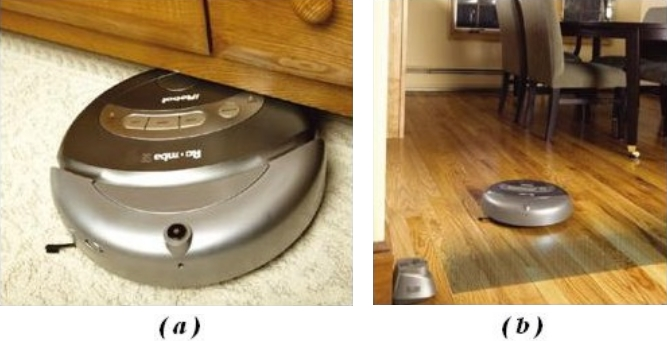
\includegraphics[width=3.4cm]{figs/roomba.jpg}
%\end{figure}
%\end{frame}

%========= Diapositiva con ítems resaltados con colores:
\begin{frame}
\frametitle{Aprendizaje colaborativo}
\begin{itemize}
\item La \textcolor{red}{tecnología} está cada vez más presente en la vida cotidiana.
\item Los robots de servicio aparecen en el \textcolor{blue}{mercado}.
\item La \textcolor{red}{domótica} presenta cada vez más aplicaciones domésticas.
\end{itemize}
\end{frame}

\subsection{Contexto específico}
%========= Diapositiva con bloques:
\begin{frame}
\frametitle{Precedentes de la robótica}
\begin{block}{Primera revolución industrial de 1800}
Productos fabricados por \textcolor{blue}{máquinas}. La \textcolor{red}{máquina de vapor} fue clave.
\end{block}
\end{frame}

%========= Diapositiva con bullets en diferentes niveles (outline):
\section{Principios de transducción}
\subsection{Principio de transducción piezoresistivo}
\begin{frame}
\frametitle{Conceptos}
\begin{outline}
\1 Piezoresistividad: relación entre resistencia eléctrica y deformación.
\2 Material piezoresistivo: (1) material en reposo (átomos en equilibrio).
\3 (2) Si sufre deformación, movimiento átomos, modifican su resistividad.
\2 Resistencia vs. resistividad de un material.
\3 Resistencia: depende del volumen del material a tratar.
\3 Resistividad: caract. intrínseca relacionada con colocación de átomos.
\end{outline}
\end{frame}

\section*{}
\begin{frame}{}
  \centering \Huge
  \emph{Objetivos}
\note[item]{Pasemos ahora a comentar los objetivos que nos hemos con este trabajo.}
\end{frame}

\section{Objetivos}
\begin{frame}
\begin{enumerate}
\item Crear una herramienta multiplataforma.
\item Sin necesidad de instalación.
\item Toda ejecución vía web.
\end{enumerate}
\end{frame}

\section*{}
\begin{frame}{}
  \centering \Huge
  \emph{Diseño}
\note[item]{Una vez descritos los objetivos, veamos qué hemos hecho para alcanzarlos.}
\end{frame}

\section{Diseño}
%========= Diapositiva con matemáticas:
\subsection{Matemáticas empleadas}
\begin{frame}
\frametitle{Matrices de la cámara}
\begin{itemize}
\item Se usa una matriz $RT (4x4)$ en lugar de $R$ y $T$.
\item La matriz $RT$ rota $\theta$ grados en los ejes $X$, $Y$ y $Z$:
\end{itemize}
\begin{equation}
	\begin{bmatrix}
	1 & 0 & 0 & X \\
	0 & cos(\theta) & sin(\theta) &	Y \\
	0 & -sin(\theta)& cos(\theta) & Z \\
	0 & 0 & 0 & 1 
	\end{bmatrix}
\end{equation}
\end{frame}

%========= Diapositiva con matemáticas y leyenda (conditions*):
\begin{frame}
\frametitle{Resistencia de un material}
\begin{outline}
\1 Si material piezoresistivo se deforma, cambia su resistencia eléctrica.
\begin{equation}
R=\rho\frac{l}{A}
\end{equation}
donde:
\begin{conditions*}
R & resistencia del material $[\Omega]$\\
\rho & resistividad $[\Omega-m]$\\
l & longitud $[m]$\\
A & área de sección transversal $[m^2]$
\end{conditions*}
\1 El cambio de resistencia se obtiene a partir de:
\begin{equation}
\frac{\Delta R}{R}=\frac{\Delta\rho}{\rho}=\frac{\Delta A}{A}=\frac{\Delta l}{l}
\end{equation}
\1 Otra forma de medir el efecto piezoresistivo: el factor de deformación.
\begin{equation}
GF(\textit{Gauge Factor})=\frac{\frac{\Delta R}{R}}{\varepsilon}=\frac{\frac{\Delta R}{R}}{\frac{\Delta l}{l}}
\end{equation}
\end{outline}
\end{frame}

%========= Diapositiva con códigos:
\subsection{Algoritmo principal}
\begin{frame}[fragile]
\frametitle{Algoritmo de visión}
\begin{lstlisting}
cvCvtColor (&image, IplTmp1, CV_RGB2GRAY);//to Gray
cvNormalize(IplTmp1, IplTmp1, 0, 255, CV_MINMAX);
cvSmooth(IplTmp1,IplTmp2,CV_BLUR,3,3);//Avrg filter
cvLaplace(IplTmp2, IplLaplace, 3);//Laplace
cvConvertScale(IplLaplace,IplTmp1);
cvThreshold(IplTmp1,IplTmp2,Thress,255,CV_THRESH_BIN);
\end{lstlisting}
\end{frame}

\section*{}
\begin{frame}{}
  \centering \Huge
  \emph{Conclusiones}
\note[item]{Para acabar esta presentación, vamos a repasar lo hecho, unas breves conclusiones y las líneas futuras.}
\end{frame}

\section{Conclusiones}
\begin{frame}
\begin{block}{Objetivos cumplidos}
\begin{itemize}
\item Herramienta multiplataforma: soporta Linux, Windows, MacOS.
\item Intuitiva para el usuario final: no se necesita instalar nada.
\item Solo se necesita un navegador web.
\end{itemize}
\end{block}

\begin{block}{Líneas futuras}
\begin{itemize}
\item Permitir el uso de otras herramientas.
\item Ampliar los botones disponibles en el interfaz.
\end{itemize}
\end{block}
\end{frame}

\begin{frame}[plain]
\large{\titlepage}
\note[item]{Y hasta aquí mi exposición.}
\note[item]{Quedo a disposición del tribunal...}
\end{frame}

\end{document}
